% Options for packages loaded elsewhere
\PassOptionsToPackage{unicode}{hyperref}
\PassOptionsToPackage{hyphens}{url}
%
\documentclass[
]{article}
\usepackage{lmodern}
\usepackage{amssymb,amsmath}
\usepackage{ifxetex,ifluatex}
\ifnum 0\ifxetex 1\fi\ifluatex 1\fi=0 % if pdftex
  \usepackage[T1]{fontenc}
  \usepackage[utf8]{inputenc}
  \usepackage{textcomp} % provide euro and other symbols
\else % if luatex or xetex
  \usepackage{unicode-math}
  \defaultfontfeatures{Scale=MatchLowercase}
  \defaultfontfeatures[\rmfamily]{Ligatures=TeX,Scale=1}
\fi
% Use upquote if available, for straight quotes in verbatim environments
\IfFileExists{upquote.sty}{\usepackage{upquote}}{}
\IfFileExists{microtype.sty}{% use microtype if available
  \usepackage[]{microtype}
  \UseMicrotypeSet[protrusion]{basicmath} % disable protrusion for tt fonts
}{}
\makeatletter
\@ifundefined{KOMAClassName}{% if non-KOMA class
  \IfFileExists{parskip.sty}{%
    \usepackage{parskip}
  }{% else
    \setlength{\parindent}{0pt}
    \setlength{\parskip}{6pt plus 2pt minus 1pt}}
}{% if KOMA class
  \KOMAoptions{parskip=half}}
\makeatother
\usepackage{xcolor}
\IfFileExists{xurl.sty}{\usepackage{xurl}}{} % add URL line breaks if available
\IfFileExists{bookmark.sty}{\usepackage{bookmark}}{\usepackage{hyperref}}
\hypersetup{
  pdftitle={APLS study},
  hidelinks,
  pdfcreator={LaTeX via pandoc}}
\urlstyle{same} % disable monospaced font for URLs
\usepackage[margin=1in]{geometry}
\usepackage{longtable,booktabs}
% Correct order of tables after \paragraph or \subparagraph
\usepackage{etoolbox}
\makeatletter
\patchcmd\longtable{\par}{\if@noskipsec\mbox{}\fi\par}{}{}
\makeatother
% Allow footnotes in longtable head/foot
\IfFileExists{footnotehyper.sty}{\usepackage{footnotehyper}}{\usepackage{footnote}}
\makesavenoteenv{longtable}
\usepackage{graphicx,grffile}
\makeatletter
\def\maxwidth{\ifdim\Gin@nat@width>\linewidth\linewidth\else\Gin@nat@width\fi}
\def\maxheight{\ifdim\Gin@nat@height>\textheight\textheight\else\Gin@nat@height\fi}
\makeatother
% Scale images if necessary, so that they will not overflow the page
% margins by default, and it is still possible to overwrite the defaults
% using explicit options in \includegraphics[width, height, ...]{}
\setkeys{Gin}{width=\maxwidth,height=\maxheight,keepaspectratio}
% Set default figure placement to htbp
\makeatletter
\def\fps@figure{htbp}
\makeatother
\setlength{\emergencystretch}{3em} % prevent overfull lines
\providecommand{\tightlist}{%
  \setlength{\itemsep}{0pt}\setlength{\parskip}{0pt}}
\setcounter{secnumdepth}{-\maxdimen} % remove section numbering

\title{APLS study}
\author{}
\date{\vspace{-2.5em}}

\begin{document}
\maketitle

{
\setcounter{tocdepth}{2}
\tableofcontents
}
Total mothers

\begin{verbatim}
## [1] 92
\end{verbatim}

\begin{verbatim}
##   total_pregnancies
## 1               373
\end{verbatim}

Checking for clinical criteria

\begin{verbatim}
## # A tibble: 4 x 2
##   criterion     n
##   <chr>     <int>
## 1 1            64
## 2 2             1
## 3 3            14
## 4 no           13
\end{verbatim}

After correcting for criteria

\begin{longtable}[]{@{}rr@{}}
\toprule
Total.mothers & Total.pregnancie\tabularnewline
\midrule
\endhead
79 & 317\tabularnewline
Treatment &\tabularnewline
\bottomrule
\end{longtable}

\begin{verbatim}
##   Aspirin_only LMWH_only Either None Both Aspirin LMWH
## 1           25         9     68  249   34      59   43
\end{verbatim}

demography

number of pregnancies

\begin{verbatim}
##   0%  25%  50%  75% 100% 
##    1    3    4    5    9
\end{verbatim}

PIH

\begin{verbatim}
##   PIH percent - out of pregnancies
## 1  17                     5.362776
\end{verbatim}

Other Medical conditions

\begin{verbatim}
## # A tibble: 1 x 3
##   condition          n `percent - out of mothers`
##   <chr>          <int>                      <dbl>
## 1 Hypothyroidism     2                       2.17
\end{verbatim}

Investigations Any of the 5 investigations

\begin{verbatim}
## # A tibble: 1 x 2
##   `Any investigation` `precent - of mothers`
##                 <dbl>                  <dbl>
## 1                  26                   32.9
\end{verbatim}

Any of Lupus, APLS, cardiolipin, beta2

Proportion of a positive result

\begin{verbatim}
## # A tibble: 1 x 2
##   `Any investigation out of Lupus, cardio, beta, APLS` `precent - of mothers`
##                                                  <dbl>                  <dbl>
## 1                                                   25                   31.6
\end{verbatim}

\begin{verbatim}
## # A tibble: 1 x 2
##   `positive subjects` `percent of tested`
##                 <dbl>               <dbl>
## 1                  11                  44
\end{verbatim}

Previous pregnancy outcome without specific treatment

\begin{longtable}[]{@{}rrrrrr@{}}
\toprule
Total & Successful & failed.pregnancies & success.rate & MC.before.10.wk
& MC.at.or.after.10.wk\tabularnewline
\midrule
\endhead
249 & 37 & 212 & 14.85944 & 90 & 113\tabularnewline
\bottomrule
\end{longtable}

Previous pregnancy outcome - Treated by either Aspirin or LMWH

\begin{longtable}[]{@{}rrrrrr@{}}
\toprule
total.pregnancies & successful.pregnancies & failed.pregnancies &
success.rate & MC.before.10.wk & MC.at.or.after.10.wk\tabularnewline
\midrule
\endhead
68 & 33 & 35 & 48.52941 & 6 & 28\tabularnewline
\bottomrule
\end{longtable}

Previous pregnancy outcome - Treated Aspirin and LMWH

\begin{longtable}[]{@{}rrrrrr@{}}
\toprule
total.pregnancies & successful.pregnancies & failed.pregnancies &
success.rate & MC.before.10.wk & MC.at.or.after.10.wk\tabularnewline
\midrule
\endhead
34 & 23 & 11 & 67.64706 & 3 & 7\tabularnewline
\bottomrule
\end{longtable}

Previous pregnancy outcome - Treated Aspirin alone

\begin{longtable}[]{@{}rrrrrr@{}}
\toprule
total.pregnancies & successful.pregnancies & failed.pregnancies &
success.rate & MC.before.10.wk & MC.at.or.after.10.wk\tabularnewline
\midrule
\endhead
25 & 5 & 20 & 20 & 3 & 17\tabularnewline
\bottomrule
\end{longtable}

Previous pregnancy outcome - Treated LMWH alone

\begin{longtable}[]{@{}rrrrrr@{}}
\toprule
total.pregnancies & successful.pregnancies & failed.pregnancies &
success.rate & MC.before.10.wk & MC.at.or.after.10.wk\tabularnewline
\midrule
\endhead
9 & 5 & 4 & 55.55556 & 0 & 4\tabularnewline
\bottomrule
\end{longtable}

comparison

No treatment vs any

\begin{verbatim}
## # A tibble: 1 x 9
##   estimate1 estimate2 statistic p.value parameter conf.low conf.high method
##       <dbl>     <dbl>     <dbl>   <dbl>     <dbl>    <dbl>     <dbl> <chr> 
## 1     0.485     0.149      33.3 4.02e-9         1    0.221         1 2-sam~
## # ... with 1 more variable: alternative <chr>
\end{verbatim}

No treatment vs both

\begin{verbatim}
## # A tibble: 1 x 9
##   estimate1 estimate2 statistic  p.value parameter conf.low conf.high method
##       <dbl>     <dbl>     <dbl>    <dbl>     <dbl>    <dbl>     <dbl> <chr> 
## 1     0.676     0.149      46.8 3.96e-12         1    0.374         1 2-sam~
## # ... with 1 more variable: alternative <chr>
\end{verbatim}

No treatment vs asp

\begin{verbatim}
## # A tibble: 1 x 9
##   estimate1 estimate2 statistic p.value parameter conf.low conf.high method
##       <dbl>     <dbl>     <dbl>   <dbl>     <dbl>    <dbl>     <dbl> <chr> 
## 1       0.2     0.149     0.151   0.349         1   -0.107         1 2-sam~
## # ... with 1 more variable: alternative <chr>
\end{verbatim}

No treatment vs LMWH

\begin{verbatim}
## # A tibble: 1 x 9
##   estimate1 estimate2 statistic p.value parameter conf.low conf.high method
##       <dbl>     <dbl>     <dbl>   <dbl>     <dbl>    <dbl>     <dbl> <chr> 
## 1     0.556     0.149      7.78 0.00264         1   0.0744         1 2-sam~
## # ... with 1 more variable: alternative <chr>
\end{verbatim}

ASP treatment vs LMWH

\begin{verbatim}
## # A tibble: 1 x 9
##   estimate1 estimate2 statistic p.value parameter conf.low conf.high method
##       <dbl>     <dbl>     <dbl>   <dbl>     <dbl>    <dbl>     <dbl> <chr> 
## 1     0.556       0.2      2.50   0.114         1  -0.0805     0.792 2-sam~
## # ... with 1 more variable: alternative <chr>
\end{verbatim}

ASP treatment vs both

\begin{verbatim}
## # A tibble: 1 x 9
##   estimate1 estimate2 statistic p.value parameter conf.low conf.high method
##       <dbl>     <dbl>     <dbl>   <dbl>     <dbl>    <dbl>     <dbl> <chr> 
## 1     0.676       0.2      11.3 3.93e-4         1    0.255         1 2-sam~
## # ... with 1 more variable: alternative <chr>
\end{verbatim}

LMWH treatment vs both

\begin{verbatim}
## # A tibble: 1 x 9
##   estimate1 estimate2 statistic p.value parameter conf.low conf.high method
##       <dbl>     <dbl>     <dbl>   <dbl>     <dbl>    <dbl>     <dbl> <chr> 
## 1     0.676     0.556    0.0804   0.388         1   -0.252         1 2-sam~
## # ... with 1 more variable: alternative <chr>
\end{verbatim}

~\\

\hypertarget{results}{%
\paragraph{results}\label{results}}

A total of 317 pregnancies were evaluated of 79 mothers. The median
number of pregnancies was 4 with an inter-quantile range of 2.
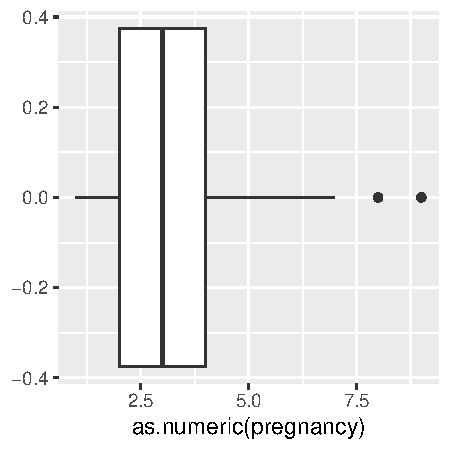
\includegraphics{Figs/unnamed-chunk-27-1.pdf} The mean age of the
selected mothers was 32.2051282 with a standard deviation of 5.1278688.
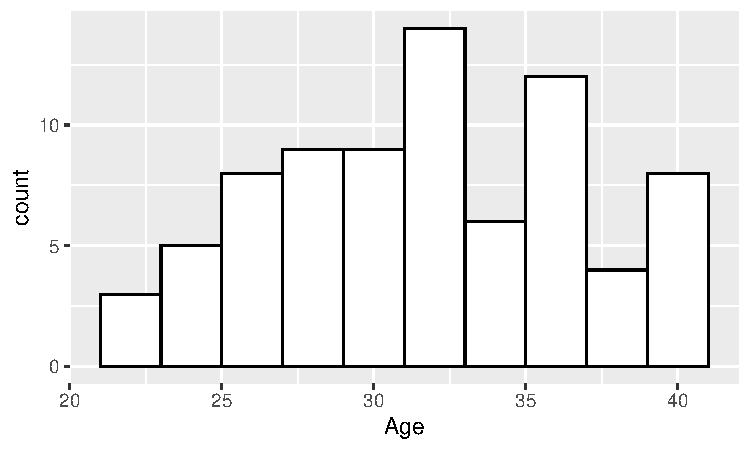
\includegraphics{Figs/unnamed-chunk-28-1.pdf}

34 pregnancies were treated with both LMWH and aspirin. 25 and 9
pregnancies were treated with aspirin alone and LMWH alone,
respectively.

~ 17 pregnancies were complicated with PIH.

\begin{verbatim}
##   PIH percent - out of pregnancies
## 1  17                     5.362776
\end{verbatim}

Outcome by treatment group 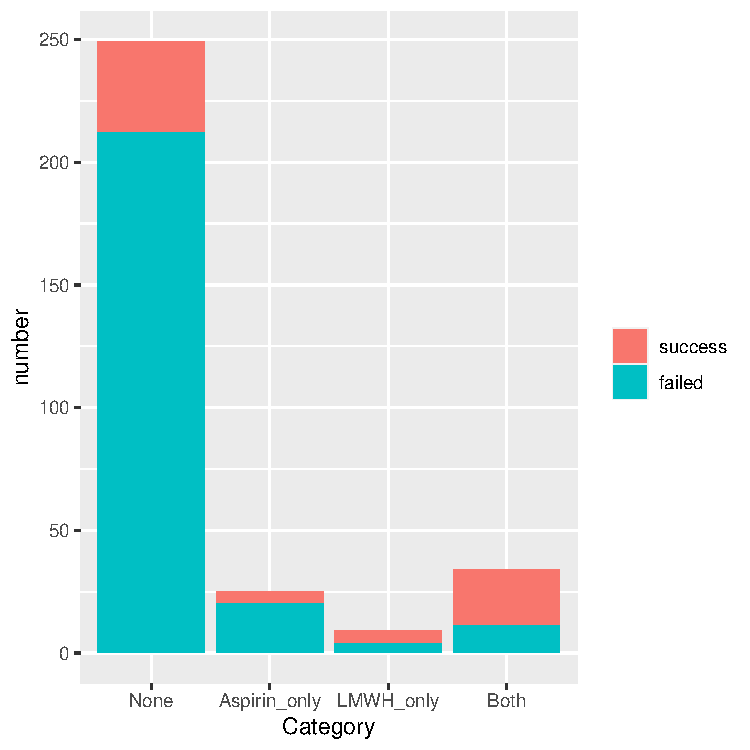
\includegraphics{Figs/unnamed-chunk-30-1.pdf}

The rate of live births among mothers who were not received specific
treatment for APS was 0.1485944. In contrast, 68 gestations were treated
with either aspirin, LMWH or both and the rate of successful outcome was
0.4852941

Outcome in each group is summarized below

\begin{longtable}[]{@{}lrrr@{}}
\toprule
Category & n & live births & live birth rate\tabularnewline
\midrule
\endhead
None & 249 & 37 & 14.85944\tabularnewline
Aspirin only & 25 & 5 & 20.00000\tabularnewline
LMWH only & 9 & 5 & 55.55556\tabularnewline
Both & 34 & 23 & 67.64706\tabularnewline
\bottomrule
\end{longtable}

Investigations\\
25 (31.6455696\%) mothers had undergone any of antibody tests for APL
and out of them, 11 (44\%) yeilded a positive result.

\begin{longtable}[]{@{}rrrr@{}}
\toprule
Lupus & cardiolipin & beta 2 microglobulin & APL\tabularnewline
\midrule
\endhead
22 & 19 & 5 & 6\tabularnewline
\bottomrule
\end{longtable}

Live rates between test positives and negatives

Number of pregnancies that were treated, in mothers who were tested for
antibodies was 19. Out of them, 10 (52.6315789\%) mothers tested
positive for at least one test and the success rate was 0.2. 9
(47.3684211\%) mothers had negative results and success rate among them
was 0.2222222

~~

\end{document}
